% !TEX root = tarasov-qasp-zh.tex

\chapter[你知道阿基米德原理吗？]{你知道阿基米德原理吗？\label{ch-16}}

\begin{dialogue}

\tchr 你知道阿基米德原理（Archimedes' principle）吗？

\stda 当然知道。液体对浸在其中的物体所施加的浮力（buoyant force），恰好等于物体所排开的液体的重力。

\tchr 对。只是还应当把它推广，把气体也包括进来：气体对“浸”在它里面的物体同样施加浮力。那么，你能为你的这个说法给出一个理论证明吗？
\pnote{浮力与阿基米德原理在中国是初中内容：人教版初中物理八年级下册第十章《浮力》，其中第 2 节即“阿基米德原理”（浮力大小等于物体排开的液体所受的重力），第 3 节“物体的浮沉条件及应用”给出下文用到的漂浮条件；液体压强公式 $p=\rho gh$ 见同册第九章“液体的压强”一节。本问则把这条原理推到高中与竞赛层面：下面的两种推导（能量法、压强差法）都超出初中要求，却能回答原理“为什么成立”。}

\stda 给阿基米德原理作证明？

\tchr 是的。

\stda 可是，阿基米德原理是直接从实验中发现的呀。

\tchr 完全正确。不过，它也可以从简单的能量考虑推导出来。设想把一个体积为 $V$、密度为 $\rho$ 的物体举高 $H$，先在真空中，后在密度为 $\rho_{0}$ 的液体中。第一种情形所需的能量等于 $\rho g V H$。第二种情形所需的能量较少，因为在把体积为 $V$ 的物体举高 $H$ 的同时，有同样体积 $V$ 的液体下降了同一高度 $H$。因此，第二种情形所耗费的能量等于
\begin{equation*}%
\rho g V H - \rho_{0} g V H
\end{equation*}
把减项 $\rho_{0} g V H$ 看作某个力所做的功，就可以得出结论：与真空相比，液体中有一个附加的力 $F=\rho_{0} g V$ 作用在物体上，使举高它更省力。这个力就叫做浮力。十分明显，它恰好等于物体浸入液体所占据的体积 $V$ 内的液体的重力。（注意，我们忽略了物体在液体中实际移动时伴随摩擦而来的能量损耗。）
\pnote{底本此处把浮力排作 $F=\rho_{0}gVH$，量纲上站不住：$\rho_{0}gVH$ 是功（两种情形的能量差），不是力。由上下文应有 $\rho_{0}gVH=F\cdot H$，浮力为 $F=\rho_{0}gV$，与紧接的下一句“恰好等于体积 $V$ 内液体的重力”相合；中文版径改，待考原书。又，同段“有同样体积 $V$ 的液体下降”处底本衍一符号 $\rho$，径删。此外，这段能量论证隐含缓慢提升（准静态）的假设，否则还须计入物体与被搅动液体的动能。}

\begin{figure}%[-3cm]	%
\centering
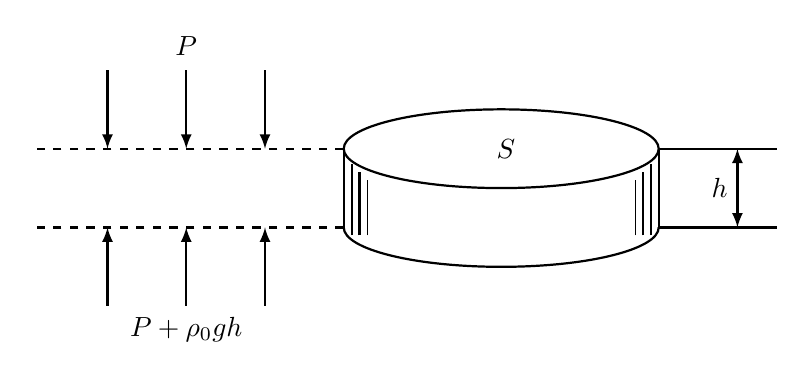
\begin{tikzpicture} [>=latex,scale=1]
\draw [thick](0,0) ellipse (2cm and 0.5cm);
\path [fill=white,](-2,0) rectangle (2,1);
\draw [fill=white,thick](0,1) ellipse (2cm and 0.5cm);
\draw [thick](-2,0) -- (-2,1);
\draw [thick](2,0) -- (2,1);
\draw [thick](1.9,-.1) -- (1.9,0.8);
\draw [thick](1.8,-.1) -- (1.8,0.7);
\draw (1.7,-.1) -- (1.7,0.6);
\draw [thick](-1.9,-.1) -- (-1.9,0.8);
\draw [thick](-1.8,-.1) -- (-1.8,0.7);
\draw (-1.7,-.1) -- (-1.7,0.6);
\draw [thick, dashed](-2,1) -- (-6,1);
\draw [thick, dashed](-2,0) -- (-6,0);
\draw [thick](2,0) -- (3.5,0);
\draw [thick](2,1) -- (3.5,1);
\draw [thick,latex-latex](3,1) -- (3,0);
\node [left] at (3,0.5) {$h$};
\node [left] at (0.3,1) {$S$};
\draw [thick,latex-](-3,0) -- (-3,-1);
\draw [thick,latex-](-4,0) -- (-4,-1);
\draw [thick,latex-](-5,0) -- (-5,-1);
\draw [thick,latex-](-3,1) -- (-3,2);
\draw [thick,latex-](-4,1) -- (-4,2);
\draw [thick,latex-](-5,1) -- (-5,2);
\node at (-4,2.3) {$P$};
\node at (-4,-1.3) {$P+\rho_{0}gh$};
\end{tikzpicture}
%\includegraphics[width=0.8\linewidth]{fig-066a.pdf}
\caption[阿基米德原理的浮力。]{阿基米德原理的浮力。\label{fig-67}}
\end{figure}
阿基米德原理也可以用稍许不同的方法导出。设浸入液体的物体是高为 $h$、底面积为 $S$ 的圆柱体（\figr{fig-67}），并设其上底面所受的压强为 $p$。

于是，下底面所受的压强将等于 $p+\rho_{0}gh$。这样，上、下两底面的压强差等于 $\rho_{0}gh$。把这个压强差乘以底面积 $S$，就得到力 $F=\rho_{0}ghS$，它力图把物体向上推。由于 $hS=V$，即圆柱体的体积，容易看出，这正是阿基米德原理中的那个浮力。
\pnote{底本这一段两处把液体密度排作 $\rho$（下底面压强 $p+\rho gh$、向上的力 $F=\rho ghS$），与前后文及\figr{fig-67} 图中标记的 $\rho_{0}$ 不一致（$\rho$ 是物体的密度，若按 $\rho$ 计算，得到的就不是浮力），中文版径改为 $\rho_{0}$，待考原书。这一“上下表面压强差”的推导，正是初中教材说明浮力产生原因的方法：浸没物体的下表面深度更大、压强更大，两个压力的差便指向上方。}

\stda 是的，现在我明白了，单凭纯粹的逻辑推理也能得出阿基米德原理。

\tchr 在继续讲下去之前，我们先来回顾一下物体的漂浮条件。

\stda 我记得这个条件：物体的重力应当被按阿基米德原理作用在物体上的浮力所平衡。

\tchr 完全正确。给你一个例子。\hlred{一块冰浮在盛水的容器里。冰熔化后，水面会变化吗？}

\stda 水面将保持不变，因为冰的重力与浮力相平衡，因而等于冰所排开的水的重力。冰熔化变成水后，其体积恰好等于先前被排开的水的体积。
\pnote{注意这个结论的前提：容器里盛的恰好是水，冰熔化所得的也是水，二者密度相同。若冰浮在密度更大的液体（如海水，约 $1.025\times10^{3}~\mathrm{kg/m^{3}}$）上，则漂浮时排开液体的重力等于冰的重力，而熔成的淡水密度较小、体积较大，液面将略微上升——升幅约为所排开液体体积的 $2.5\%$，海冰熔化使海平面微升的道理即在于此（当然，海平面上升的大头是陆地冰）。“液面不变”只属于“冰浮于水”这一情形。}

\tchr 正是如此。现在假定冰里包着一块铅。在这种情形下，冰熔化后水面会怎样？

\stda 我不大有把握，不过我想水面应当略有下降。可是我证明不了。

\tchr 我们把冰连同铅块的体积记作 $V$，铅块的体积记作 $v$，冰浸入水中的部分所排开的水的体积记作 $V_{1}$，水的密度记作 $\rho_{0}$，冰的密度记作 $\rho_{1}$，铅的密度记作 $\rho_{2}$。冰连同铅块的重力等于
\begin{equation*}%
\rho_{1} g (V-v) + \rho_{2}gv
\end{equation*}
这个重力与浮力 $\rho_{0}gV_{1}$ 相平衡。于是
\begin{equation}%
\rho_{1} g (V-v) + \rho_{2}g v = \rho_{0}g V_{1}
\label{eq-90}
\end{equation}
冰熔化后变成水，其体积 $V_{2}$ 由下方程求出：
\begin{equation*}
\rho_{1} g (V-v) = \rho_{0} gV_{2}
\end{equation*}
把这个方程代入式~\eqref{eq-90}，得
\begin{equation*}%
\rho_{0}gV_{2} + \rho_{2}gv = \rho_{0}gV_{1}
\end{equation*}
由此求得冰熔化所得到的水的体积为
\begin{equation}%
V_{2} = V_{1} -v \frac{\rho_{2}}{\rho_{0}}
\label{eq-91}
\end{equation}
\pnote{式~\eqref{eq-90} 右端底本排作 $\rho_{0}gVt$，$Vt$ 显系 $V_{1}$ 之误——$V_{1}$ 正是前句刚定义的量，且下文“把这个方程代入式~\eqref{eq-90}”所得的结果中也是 $\rho_{0}gV_{1}$；式~\eqref{eq-91} 底本分母排作 $\rho_{1}$，应为 $\rho_{0}$：由它推出的式~\eqref{eq-92} 与后文软木情形借用的式~\eqref{eq-94} 都只与 $\rho_{0}$ 相洽。中文版均径改，待考原书。}
可见，冰熔化前，被排开的水的体积是 $V_{1}$；熔化之后，铅块和冰化成的水开始占据体积 $(V_{2}+v)$。要回答容器中水面如何变化的问题，应当比较这两个体积。由式~\eqref{eq-91} 得
\begin{equation}%
V_{2} + v= V_{1} - v \frac{\rho_{2}-\rho_{0}}{\rho_{0}}
\label{eq-92}
\end{equation}
由于 $\rho_{2}>\rho_{0}$（铅比水重），由式~\eqref{eq-92} 可以看出 $(V_{2}+v)<V_{1}$。因此，冰熔化的结果是水面将下降。把体积差 $V_{1}-(V_{2}+v)$ 除以容器的横截面积 $S$（为简单起见，设容器呈圆柱形），即可求出冰熔化后水面下降的高度 $h$。于是
\begin{equation}%
h= v \left( \frac{\rho_{2}-\rho_{0}}{\rho_{0}S} \right)
\label{eq-93}
\end{equation}
这个题的解法你明白了吗？

\stda 是的，我完全明白了。

\tchr 那么，把铅块换成一块体积为 $v$、密度为 $\rho_{3}$ 的软木块封进冰里。冰熔化后水面会怎样？

\stda 我想水面会略微上升。

\tchr 为什么？

\stda 在铅的例子中水面下降了。铅比水重，而软木比水轻。因此，在软木的情形应当预期相反的效果：水面应当上升。

\tchr 你错了。要是冰熔化后软木块仍处于浸没状态，你的回答就对了。可是软木比水轻，它必定会升到水面上并漂浮起来。因此，软木（以及任何别的比水轻的物体）的例子需要专门考虑。利用式~\eqref{eq-91} 的结果，可以求出冰连同软木块所排开的水的体积与冰熔化所得到的水的体积之差。于是
\begin{equation}%
V_{1} - V_{2} = v \left( \frac{\rho_{3}}{\rho_{0}} \right)
\label{eq-94}
\end{equation}
再对软木块应用漂浮条件：
\begin{equation}%
\rho_{3}v  = \rho_{0}v_{1}
\label{eq-95}
\end{equation}
其中 $v_{1}$ 是软木块浸入水中的那部分的体积。把这个方程代入式~\eqref{eq-94}，得
\begin{equation*}%
V_{1} = V_{2} +v_{1}
\end{equation*}
这样，\hlblue{冰块所排开的水的体积，恰好等于冰熔化所得到的水的体积与漂浮的软木块浸没部分所排开的水的体积之和。所以在这种情形下水面保持不变。}

\stda 要是冰里封的不是软木块，而只是一个气泡呢？

\tchr 冰熔化后，气泡会逸出。容易看出，容器中的水面将与冰熔化前完全相同。简言之，冰里含气泡的例子与含软木块的例子是类似的。
\pnote{“液面升降”类问题的统一要领：比较变化前被排开的液体体积与变化后各物体实际占据的体积。含气泡的冰相当于软木块情形的极限：气泡密度趋于零，由式~\eqref{eq-95}，其漂浮时排开的体积 $v_{1}\to 0$，于是 $V_{1}=V_{2}$，液面不变，与教师的结论相合。铅（沉底）、软木（漂浮）、气泡（逸出）三种情形，正好覆盖了这类问题的全部基本类型。}

\stda 我看，以阿基米德原理为基础，可以编出许多很有意思的问题和习题。

\tchr 遗憾的是，一些考生在准备物理考试时对这条原理重视不够。来看下面的例子。\hlred{天平的一只秤盘上放着盛水的容器，另一只秤盘上放着一个支架，支架上悬挂着一个重物，两盘相互平衡（\figr{fig-68}~\drkgry{(a)}）。然后转动支架，使悬挂的重物完全没入水中。显然，平衡被破坏了，因为放支架的秤盘变轻了（\figr{fig-68}~\drkgry{(b)}）。要恢复平衡，必须在放支架的秤盘上加放多大的重物？}

\begin{figure}
\centering
\includegraphics[width=0.5\textwidth,angle=-2]{figs/ch-16/fig-068a}
\caption[恢复平衡所需加放的重物。]{必须在天平放支架的秤盘上加放多大的重物，才能恢复平衡？\label{fig-68}}
\end{figure}

\stda 没入水中的重物受到一个浮力，其大小等于被重物排开的那部分水的重力（我们把这部分水的重力记作 $P$）。因此，要恢复平衡，应在放支架的秤盘上放一个重力为 $P$ 的重物。

\tchr 你错了。你最好回想一下牛顿第三定律。根据这条定律，容器中的水作用在没入重物上的力，与没入的重物沿相反方向作用在水上的力大小精确相等。因此，在放支架的秤盘变轻的同时，放容器的秤盘变重了。所以，要恢复平衡，应在放支架的秤盘上加放重力等于 $2P$ 的重物。
\pnote{只答 $P$、漏掉水所受反作用力的另一半，是这道经典题的典型错误。牛顿第三定律见人教版必修第一册第三章“相互作用——力”。同类常见变式：台秤上放盛水烧杯，把手指浸入水中（不碰杯壁与杯底），台秤示数增大——手指所受浮力的反作用力经水传到杯底。本题不过是把一对相互作用力分置于天平两盘，故差额为 $2P$。}

\stda 我不大明白您的推理。要知道，重物与水的这种相互作用，怎么也不像力学中两个物体之间的相互作用呀。

\tchr 牛顿第三定律的适用范围不限于力学。“对每一个作用，都有一个大小相等、方向相反的反作用”这句话，涉及许许多多种相互作用。不过，在我们这个情形里，可以换一种你肯定不会反对的论证。我们把带重物的支架和盛水的容器看作同一个系统的两个部分，系统的总重力显然等于左、右两盘重力之和。系统各部分彼此之间的相互作用不应改变系统的总重力。因此，如果相互作用的结果使右盘变轻了 $P$，左盘就必定加重同一个量（$P$）。于是，重物没入水中之后，左、右两盘重力之差应为 $2P$。
\pnote{这段“系统论证”就是第 2 章处理物体系统时用过的整体法（见\chap{ch-02}）：内力成对出现，不改变系统的总量——那里是“内力不出现在整体的运动方程中”，这里是“内力不改变系统的总重力”。到大学普通物理中，这一思想统一表述为“内力成对抵消，对系统总动量没有贡献”。}

\end{dialogue}

\section*{习题}
\label{prob-16}
\addcontentsline{toc}{section}{习题}


\begin{enumerate}[resume*=problems]
\item 圆柱形容器的横截面积为 $S$，其中盛着水，水里浮着一块内含铅球的冰。冰连同铅球的体积为 $V$，该体积的 $1/20$ 露出水面。冰熔化后，容器中的水面将下降到哪条标线？设水、冰、铅的密度均为已知。


\end{enumerate}


\cleardoublepage

% NEWTERMS: Archimedes' principle | 阿基米德原理 | 正文首现于本章（括注英文）；ch-15-zh 章尾格言先出现但未括注（彼处 NEWTERMS 已声明"正文将于下一章起展开"），ch-17-zh 另作首现括注并声明归属待本章定，全书收尾时撤彼处括注
% NEWTERMS: buoyant force | 浮力 | 首现括注；人教版初中八年级下册第十章《浮力》；首现归属同上
% NEWTERMS: liquid displaced | 被排开的液体 | 原理表述作"物体所排开的液体的重力"（人教版表述"排开的液体所受的重力"）；ch-17-zh 同一表述作"重量"，冲突备案，全书收尾统一
% NEWTERMS: density | 密度 | 基础术语不括注 |
% NEWTERMS: pressure | 压强 | 基础术语不括注；本章用于上下底面压强差推导，系统展开见后续流体静力学各章（ch-17-zh 已备案，首现实归本章）
% NEWTERMS: upper / lower base | 上底面／下底面 | 圆柱体语境；ch-17 承本章
% NEWTERMS: condition for the floating of a body | 漂浮条件 | 对接初中"物体的浮沉条件"
% NEWTERMS: melt | 熔化 | 冰变为水；教材作"熔化"不作"融化"
% NEWTERMS: water level | 水面 | 液面升降类问题语境
% NEWTERMS: submerged / immersed | 没入／浸在……中 | 本章"完全没入水中""浸在其中的物体"；与 ch-17 的"浸没"同义，全书收尾统一
% NEWTERMS: lead | 铅 | |
% NEWTERMS: piece of cork | 软木块 | 密度 $\rho_{3}$、体积 $v$、$v_{1}$，ch-17 承本章符号
% NEWTERMS: bubble of air | 气泡 | |
% NEWTERMS: balance / pan | 天平／秤盘 | |
% NEWTERMS: stand | 支架 | 可转动并悬挂重物
% NEWTERMS: weight (object on pan) | 重物 | 天平语境的物质对象；物理量 weight 依第 2、9 章处理（本章力图语境译"重力"）
% NEWTERMS: vessel | 容器 | |
% NEWTERMS: examinee | 考生 | 承前言语境（高校入学考试）
